\documentclass[a4paper,12pt,oneside,pdflatex,italian,final,twocolumn]{article}

\usepackage[utf8]{inputenc}
\usepackage{parallel}
\usepackage{siunitx}
\usepackage{booktabs}
\usepackage{fancyhdr}
\usepackage{subcaption}
\usepackage{minted}
\usepackage{hyperref}
\usepackage{pdfpages}

\usepackage[export]{adjustbox}
\usepackage[margin=0.5in]{geometry}
\addtolength{\topmargin}{0in}

\usepackage{libertine}
\renewcommand*\familydefault{\sfdefault}  %% Only if the base font of the document is to be sans serif
\usepackage[T1]{fontenc}

\hypersetup{
	colorlinks=true, %set true if you want colored links
	linktoc=all,     %set to all if you want both sections and subsections linked
	linkcolor=blue,  %choose some color if you want links to stand out
	urlcolor=blue,   %url color
}

\definecolor{LightGray}{gray}{0.95}

\title{Custom Vibration Sensor v0}
\author{Achmadi ST MT}
\date{September 2023}

\begin{document}
	\pagestyle{fancy}
	
	\lhead{Achmadi ST MT}
	\chead{\today}
	\rhead{Specification Document}
	
	\onecolumn
	\begin{figure}
		
	\end{figure}\begin{minipage}{0.47\textwidth}
		\centering
		
	\end{minipage}
	\hfill
	\begin{minipage}{0.47\textwidth}
		\raggedleft
		\Huge \textbf{Custom ESP12F Module v0}
	\end{minipage}

\begin{figure}
	\begin{minipage}{0.47\textwidth}
		
		\section{Overview}
		\begin{itemize}
			\item Based on ESP-12F and CH340C
			\item Basic IoT module with WiFi and LED testing
			\item USB Powered with Serial USB-TTL
		\end{itemize}
		
		\end{minipage}
		\hfill
		\begin{minipage}{0.47\textwidth}
			\centering
			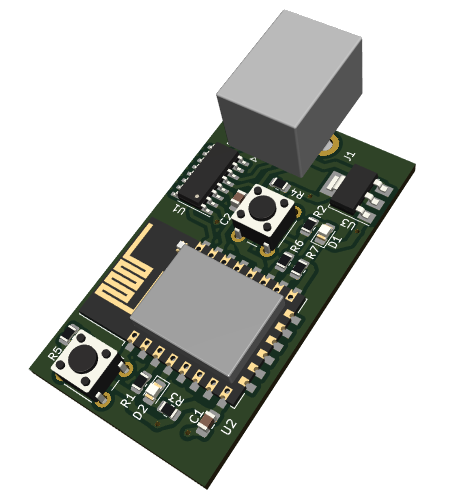
\includegraphics[width=0.8\textwidth,right]{images/perspective.png}
		\end{minipage}
	\end{figure}

	\raggedright
	
	\section{Project Repository}
	
	All Design example here can be found at: \url{https://github.com/mekatronik-achmadi/example_collection/tree/master/circuit/kicad/custom_esp12f}.
	
	\section{Board Layout}
	
	\begin{figure}[h]
		\centering
		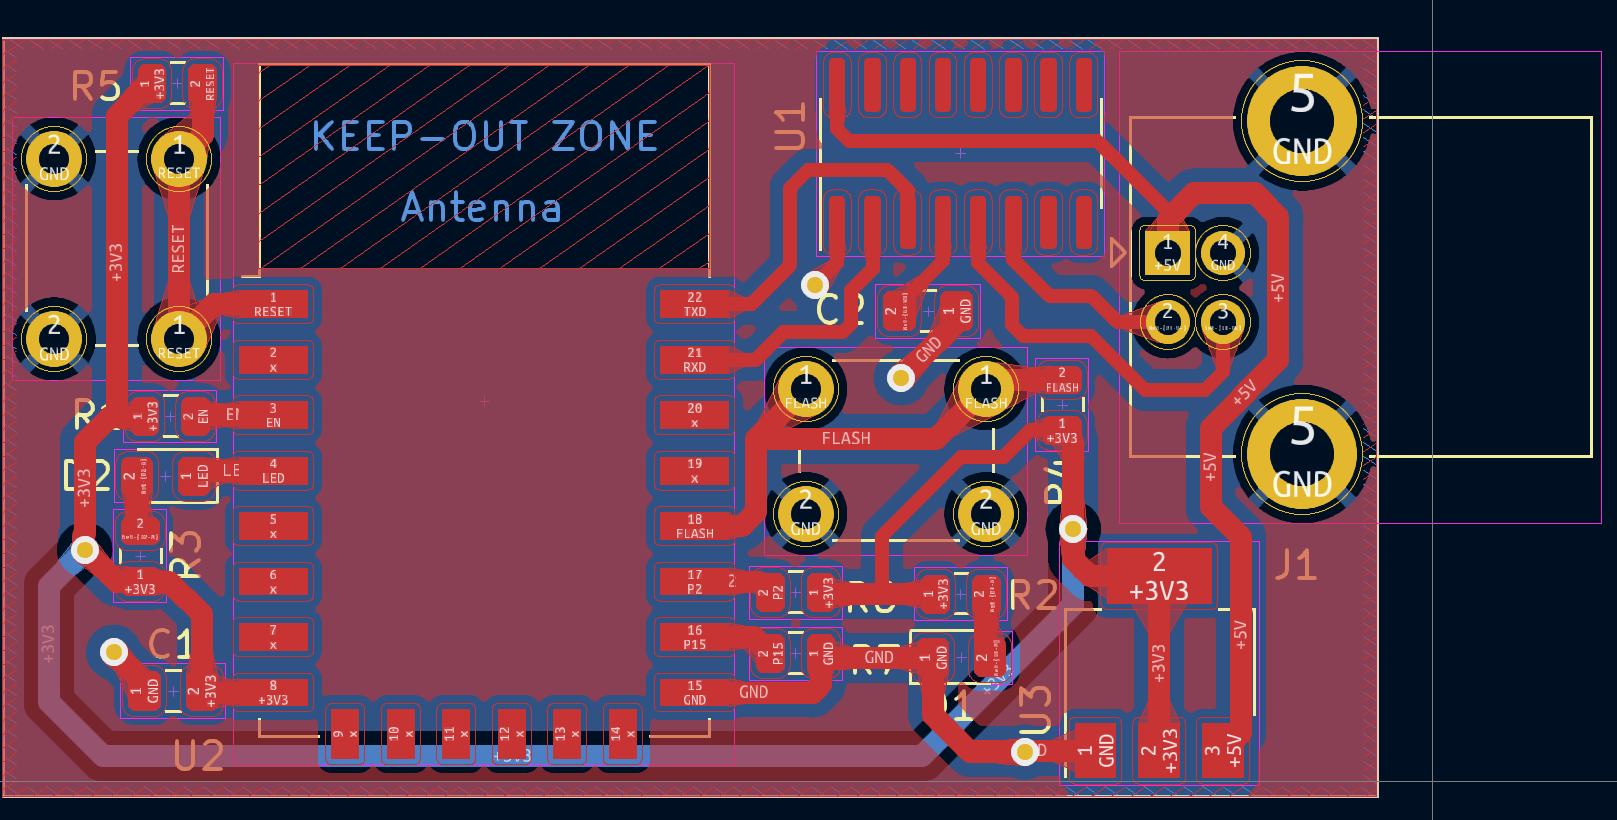
\includegraphics[width=\textwidth]{images/board.png}
		\caption{Board Layout}
	\end{figure}

	\section{Schematic Design}
	
	\newpage
	\includepdf[pages=-,angle=-90]{images/custom_esp12f.pdf}
	
	\raggedright
	
	\newpage
	\section{Unit Preview}
	\begin{figure}[h]
		\centering
		\begin{subfigure}{0.45\textwidth}
			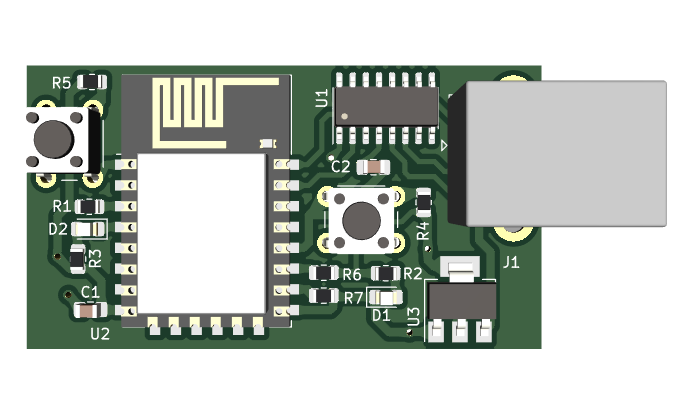
\includegraphics[width=\textwidth]{images/top.png}
			\caption{Top}
		\end{subfigure}
		\begin{subfigure}{0.45\textwidth}
			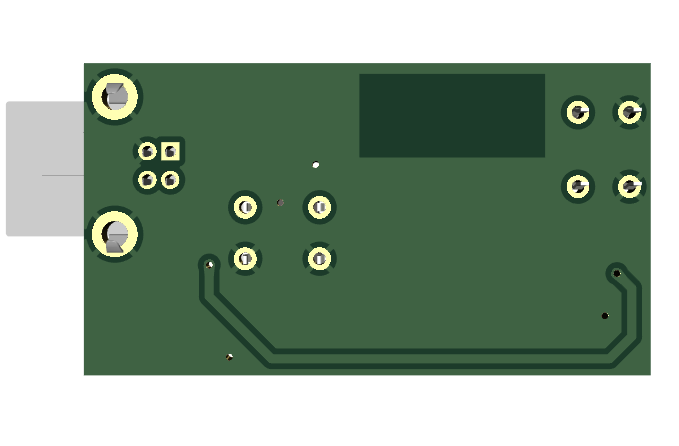
\includegraphics[width=\textwidth]{images/bottom.png}
			\caption{Bottom}
		\end{subfigure}
	\end{figure}

	\section{Bill of Material}
	
	\subsection{Components}
	
	\begin{table}[!ht]
		\centering
		\begin{tabular}{|l|l|l|l|l|}
			\hline
			Item & Value & Qty & Buy? & URL \\
			\hline
			C 0805 & 100nF & 2 & Yes & \href{https://www.tokopedia.com/ndtechnology/kapasitor-capacitor-smd-0805-100nf-bijian-pcs}{Tokopedia} \\
			R 0805 & 10K & 5 & No & \href{https://www.tokopedia.com/wiksatech/resistor-10k-5-0805-284b}{Tokopedia} \\
			R 0805 & 330 & 2 & No & \href{https://www.tokopedia.com/isee/resistor-smd-0805-330ohm-330-ohm-toleransi-1-tolerance-1}{Tokopedia} \\
			LED 0805 & - & 2 & Yes & \href{https://www.tokopedia.com/wkh-elektronik/led-smd-0805-white-color-warna-putih-smt}{Tokopedia} \\
			CH340C & - & 1 & Yes & \href{https://www.tokopedia.com/celectro/ic-ch340c-smd}{Tokopedia} \\
			ESP-12F & - & 1 & Yes & \href{https://www.tokopedia.com/cncstorebandung/cnc-esp8266-esp-12f-esp12f-esp-12-esp12-wifi-serial-transceiver}{Tokopedia} \\
			AMS1117 & 3.3v & 1 & Yes & \href{https://www.tokopedia.com/isee/ams1117-3-3v-smd-regulator-sot-223}{Tokopedia} \\
			Button & 6mm & 2 & Offline & \href{https://www.tokopedia.com/eltech-online/6x6x5h-height-tinggi-5mm-tact-switch-saklar-omten-ts-6650}{Tokopedia} \\
			USB Port & Type-B & 1 & Offline & \href{https://www.tokopedia.com/eltech-online/usb-b-pcb-female-right-angle-siku-bengkok}{Tokopedia} \\
			\hline
		\end{tabular}
	\end{table}

	\subsection{PCB Fabrications}
	
	Some recommended PCB Fabrication to be contacted:
	\begin{enumerate}
		\item Gerai Cerdas: \href{https://www.tokopedia.com/geraicerdas/cetak-pcb-1-keping-single-double-layer-rapid-prototyping-satuan}{Tokopedia}.
		
		\item Raftech: \href{https://www.tokopedia.com/raftech/jasa-cetak-pcb-double-layer-fr4-full-masking-jalur-masking-silkscreen}{Tokopedia}.
		
		\item Inovatif: \href{https://www.tokopedia.com/inovatif/cetak-pcb-satuan-dan-desain-pcb-masking}{Tokopedia}.
	\end{enumerate}

	\textbf{Notes:} This list ranked from highest price to lowest and reflect its quality.
	
\end{document}